\subsection{* 完备正则诺特局部环的结构}

本节使用第 IX 章中的定义和结果。

设 A 是正则诺特完备局部环；记其剩余域 \(\kappa_{A}\) 的特征为 p，并区分两种情形。

\begin{enumerate}
\def\labelenumi{\Alph{enumi})}
\tightlist
\item
  \(p = 0\)。则根据（IX, § 3, n° 3, 定理 1），存在 A 的子域 K，使 A 到 \(\kappa_{\mathrm{A}}\) 的典范投影将 K 同构地映到 \(\kappa_{\mathrm{A}}\)。然后将 n° 2 的定理 1 的推论 3 应用于 K-代数 A，得到：
\end{enumerate}

命题 6. --- 设 A 是正则诺特完备局部环，其剩余域 \(\kappa_{\mathrm{A}}\) 的特征为 0。置 \(n = \dim(\mathrm{A})\)。则 A 同构于形式幂级数环 \(\kappa_{\mathrm{A}}[[\mathrm{X}_{1}, ..., \mathrm{X}_{n}]]\)。

\begin{enumerate}
\def\labelenumi{\Alph{enumi})}
\setcounter{enumi}{1}
\tightlist
\item
  \(p \neq 0\)。A 的 Cohen 子环是 A 的任意子环 V，只要 V 是 \(p\)-环并满足 \(A = \mathfrak{m}_{A} + V\)（IX, § 2, no. 2, 定义 2）。环 V 是局部环；其极大理想 \(\mathfrak{m}_{V}\) 由 \(p \cdot 1_{V}\) 生成；因而有 \(\mathfrak{m}_{A} \cap V = \mathfrak{m}_{V}\)，且 V 到 A 的典范嵌入在取商后诱导出从 \(\kappa_{V}\) 到 \(\kappa_{A}\) 的域同构。若 \(p \cdot 1_{A} = 0\)，则 V 是特征为 \(p\) 的域。否则，V 是离散赋值环，其分式域的特征为 0（IX, § 2, no. 1, 命题 1 的推论 1）。已经证明（IX, no. 2, 定理 1）A 具有 Cohen 子环。
\end{enumerate}

例子。--- 1) 令 \(k\) 为特征为 \(p \neq 0\) 的域，令 \(n\) 为正整数。形式幂级数环 \(k[[X_1, ..., X_n]]\) 是维数为 \(n\) 的完备正则诺特局部环，而 \(k\) 是 \(k[[X_1, ..., X_n]]\) 的 Cohen 子环。

\begin{enumerate}
\def\labelenumi{\arabic{enumi})}
\setcounter{enumi}{1}
\item
  令 V 为完备离散赋值环，n 为正整数。形式幂级数环 \(V_{n} = V[[X_{1}, ..., X_{n}]]\) 是维数为 \(n + 1\) 的完备正则诺特局部环，而 V 是 \(V_{n}\) 的 Cohen 子环。
\item
  沿用上述记号。\(V_{n}[T]\) 中次数为 \(d \geqslant 2\) 的多项式 P 若具有如下形式 \(T^{d} + \sum_{i=1}^{d} a_{i} T^{d-i}\)，其中 \(a_{1}, \ldots, a_{d-1}\) 属于 \(m_{V_{n}}\)，\(a_{d}\) 属于 \(m_{V} + m_{V_{n}}^{2}\) 但不属于 \(m_{V_{n}}^{2}\)，则称其为特殊多项式。特别地，P 是关于 \(m_{V_{n}}\) 的艾森斯坦多项式。置 A = \(V_{n}[T]/(P)\)。根据第 4 号的命题 4 的推论，环 A 是维数为 \(n + 1\) 的完备正则诺特局部环。若 t 是 T 模 (P) 的类，则序列 \((1, t, \ldots, t^{d-1})\) 是 \(V_{n}\)-模 A 的一个基，而 \((X_{1}, \ldots, X_{n}, t)\) 是 A 的一个坐标系：事实上，存在 V 的一致化元 π，使 \(a_{d} \equiv \pi \mod m_{V_{n}}^{2}\)；又有
\end{enumerate}

\[
a _ {d} = - t \left(t ^ {d - 1} + a _ {1} t ^ {d - 2} + \dots + a _ {d - 1}\right),
\]

有 \(\pi\in\mathfrak{m}_{\mathrm{A}}^{2}\)；由于 \(\mathfrak{m}_{\mathrm{A}}\) 由 \(\{\pi,\mathrm{X}_{1},..., \mathrm{X}_{n},t\}\) 生成，这就证明了所述断言。此外，V 是 A 的一个 Cohen 子环，因为 \(\kappa_{\mathrm{V}}\) 可识别为 \(\kappa_{\mathrm{V}_{n}}\)，而 \(\kappa_{\mathrm{V}_{n}}\) 根据第 4 号命题 4 的推论可识别为 \(\kappa_{\mathrm{A}}\)。

定理 2. --- 设 A 是完备正则诺特局部环，其剩余域的特征不等于 0，且 V 是 A 的一个 Cohen 子环。置 n = dim(A)。

\begin{enumerate}
\def\labelenumi{\alph{enumi})}
\item
  假设 V 是域。则 V-代数 A 同构于形式幂级数代数 \(V[[X_{1}, ..., X_{n}]]\)。
\item
  假设 V 是完备离散赋值环，且 \(m_{V} \not\subset m_{A}^{2}\)。则 V-代数 A 同构于形式幂级数代数 \(V[[X_{1}, ..., X_{n-1}]]\)。
\item
  假设 V 是完备离散赋值环，且 \(\mathfrak{m}_{\mathrm{V}} \subset \mathfrak{m}_{\mathrm{A}}^{2}\)。则存在 \(\mathrm{V}[[\mathrm{X}_{1}, ..., \mathrm{X}_{n-1}]]\) 中的一个特殊多项式 P，属于 {[}T{]}，以及一个从 A 到 \(\mathrm{V}[[\mathrm{X}_{1}, ..., \mathrm{X}_{n-1}]]\) {[}T{]}/(P) 的 V-同构。
\end{enumerate}

断言 a) 立即由第 2 号的定理 1 的推论 3 得出。

我们证明 \(b\)。设 \((x_{1},\ldots,x_{m})\) 是 \(\mathfrak{m}_{\mathrm{A}}\) 中元素的一个序列，并令 \(\varphi_{0}\) 为从 \(\mathrm{V}[\mathrm{X}_{1},\ldots,\mathrm{X}_{m}]\) 到 A 的同态；它在 V 上为恒等，并将 \(\mathrm{X}_{i}\) 送到 \(x_{i}\)（\(1\leqslant i\leqslant m\)）。若 \(\mathfrak{a}\) 是 \(\mathrm{V}[\mathrm{X}_{1},\ldots,\mathrm{X}_{m}]\) 中由 \(\mathrm{X}_{1},\ldots,\mathrm{X}_{m}\) 生成的理想，则有 \(\varphi_{0}(\mathfrak{a})\subset\mathfrak{m}_{\mathrm{A}}\)，因而 \(\varphi_{0}\) 连续延拓为同态 \(\varphi\)，其从 \(\mathrm{V}_{m}=\mathrm{V}[[\mathrm{X}_{1},\ldots,\mathrm{X}_{m}]]\) 到 A。令 \(\pi\) 为 V 的一致化元。根据第 2 号定理 1 的推论 2，\(\varphi\) 从 \(\mathrm{V}_{m}\) 到 A 是同构，当且仅当 \((\pi,x_{1},\ldots,x_{m})\) 是 A 的一个坐标系。但是，从 \(\mathfrak{m}_{\mathrm{V}}/\mathfrak{m}_{\mathrm{V}}^{2}\) 到 \(\mathfrak{m}_{\mathrm{A}}/\mathfrak{m}_{\mathrm{A}}^{2}\) 的典范映射是单射，因为有 \(\mathfrak{m}_{\mathrm{V}}\not\subset\mathfrak{m}_{\mathrm{A}}^{2}\)，且 \(\mathfrak{m}_{\mathrm{V}}/\mathfrak{m}_{\mathrm{V}}^{2}\) 关于 \(\kappa_{\mathrm{V}}\) 的秩为 1。因此 \(\mathfrak{m}_{\mathrm{A}}/(\mathfrak{m}_{\mathrm{V}}+\mathfrak{m}_{\mathrm{A}}^{2})\) 的秩为 \(n-1\)，且 \((\pi,x_{1},\ldots,x_{m})\) 是 A 的一个坐标系，当且仅当 \(x_{i}\) 的类构成 \(\mathfrak{m}_{\mathrm{A}}/(\mathfrak{m}_{\mathrm{V}}+\mathfrak{m}_{\mathrm{A}}^{2})\) 关于 \(\kappa_{\mathrm{V}}\) 的一个基。因此 \(b)\) 得证。

我们证明 c)。设 \((y_{1}, \ldots, y_{n})\) 是 A 的一个坐标系。照上面一样，置 \(V_{n} = V[[Y_{1}, \ldots, Y_{n}]]\)，并考虑同态 \(\varphi\)，它从 \(V_{n}\) 到 A；它在 V 上为恒等，并将 \(Y_{i}\) 送到 \(y_{i}\)（\(1 \leqslant i \leqslant n\)）。于是 \(\text{gr}(\varphi)\) 是满射，故 \(\varphi\) 是满射（III, § 2, no. 8, 定理 1 的推论 2）。其核 \(\mathfrak{p}\) 是 \(\varphi\) 的核，也是 \(V_{n}\) 的素理想；由于有

\[
\dim (\mathrm{V} _ {n}) = n + 1 = \dim (\mathrm{V} _ {n} / \mathfrak {p}) + 1,
\]

素理想 p 的高度为 1（§ 1，第 3 号，命题 8）。但是，环 V \(_{n}\) 根据 VII, § 3，第 9 号的命题 8 是唯一分解环；因此理想 p 是主理想（VII, § 3，第 2 号，定理 1）。

令 R 为环 \(V_{n}\) 中理想 p 的一个生成元。根据 VII, § 3, No. 7 的引理 3，存在至少为 1 的整数 \(u(1), ..., u(n - 1)\)，以及从 \(V[[X_{1}, ..., X_{n-1}, T]]\) 到 \(V_{n}\) 的同构 σ，使得

\[
\begin{array}{l} \sigma (X _ {i}) = Y _ {i} + Y _ {n} ^ {u (i)} \quad \text { for } \quad 1 \leqslant i <   n \\ \sigma (T) = Y _ {n} \end{array}
\]

并且 \(\sigma^{-1}(R) = Q\) 满足 \(Q(0, \ldots, 0, T) \neq 0\)。此外，根据预备定理（VII, § 3, no. 8, 命题 6），存在 V{[}{[}X₁, \ldots, Xₙ₋₁{]}{]} {[}T{]} 中的多项式 P，其形状为

\[
\mathrm{P} = \mathrm{T} ^ {d} + \sum_ {i = 1} ^ {d} a _ {i} (\mathrm{X} _ {1},..., \mathrm{X} _ {n - 1}) \mathrm{T} ^ {d - i},
\]

在 \(V[[X_{1}, \ldots, X_{n-1}, T]]\) 中生成与 Q 相同理想的多项式 P，满足 \(a_{i}(0, \ldots, 0) \in \mathfrak{m}_{V}\)（\(1 \leqslant i \leqslant d\)）。由此，A 是 V-同构于 \(V[[X_{1}, \ldots, X_{n-1}, T]]/(P)\) 的。可是，\(V[[X_{1}, \ldots, X_{n-1}, T]]\) 是理想 (P) 与 \(V[[X_{1}, \ldots, X_{n-1}]]\) 的直和，后一个子模以 \(1, T, \ldots, T^{d-1}\) 为基（VII, § 3, no. 8, 命题 5）；因此，A 是 V-同构于 \(V[[X_{1}, \ldots, X_{n-1}]][T]/(P)\) 的。

置 \(C = V[[X_1, ..., X_{n-1}]]\)，记 \(\alpha\) 为 \(a_d(X_1, ..., X_{n-1})\) 模 \(m_C^2\) 的类。我们有 \(\kappa_V = \kappa_C = \kappa_A\)。根据命题 4，从 \(m_C/m_C^2\) 到 \(m_A/m_A^2\) 的典范同态的核等于 \(\kappa_C\alpha\)。由于 \(m_V/m_V^2\) 在 \(m_A/m_A^2\) 中的像为 0，且 \(m_V/m_V^2\) 关于 \(\kappa_C\) 的秩为 1，故 \(a_d\) 属于 \(m_V + m_C^2\) 但不属于 \(m_C^2\)。因此，多项式 P 是特殊多项式，这正是要证明的结论。

* 注。--- 设 \(k\) 为域，A 为完备正则诺特 \(k\)-代数。当 \(\kappa_{\mathrm{A}}\) 不是 \(k\) 的可分扩张时，一般并不成立：A 作为 \(k\)-代数同构于 \(\kappa_{\mathrm{A}}[[\mathrm{T}_{1},..., \mathrm{T}_{n}]]\)，其中 \(n = \dim(\mathrm{A})\)（p.~98, exerc. 29）。*

\pandocbounded{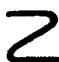
\includegraphics[keepaspectratio]{images/part001_587db9d1.jpg}}

